\documentclass[10pt, aspectratio=169]{beamer}

% Modern theme
\usetheme[progressbar=frametitle]{metropolis}
\usepackage{appendixnumberbeamer}
\usepackage{booktabs}
\usepackage[scale=2]{ccicons}
\usepackage{graphicx}
\graphicspath{{Images/}}
\usepackage{xcolor}
\usepackage{amsmath}
\usepackage{algorithm2e}

\title{Black-box Active Learning for Discovering New Explanations}
\subtitle{Application to Complex System Exploration}
\date{Derivative-Free Optimization Symposium}
\author{Paul Saves \inst{1} \and Nicolas Verstaevel \inst{1} \and Benoit Gaudou \inst{1}}
\institute{\inst{1} Université Toulouse Capitole, IRIT, France}

\begin{document}

\maketitle

\begin{frame}{Table of contents}
  \setbeamertemplate{section in toc}[sections numbered]
  \tableofcontents[hideallsubsections]
\end{frame}

\section{Introduction \& Context}

\begin{frame}[fragile]{The Computational Bottleneck of ABMs}
  \textbf{Exploring Agent-Based Models (Schelling, Cireco):}
  \begin{itemize}
    \item \textbf{Computational Expense:} A single simulator run takes significant time. High-dimensional mapping via LHS is intractable.
    \item \textbf{Black-Box \& Non-Differentiable:} No gradients to guide the search towards interesting behaviors.
    \item \textbf{The "Needle in a Haystack":} Traditional Active Learning minimizes \textit{prediction uncertainty}, wasting simulations in noisy but homogeneous regions while missing critical tipping points.
  \end{itemize}
\end{frame}

\begin{frame}[fragile]{Motivation: Tipping Points in Dual Spaces}
  \textbf{Goal:} Identify critical phase transitions in both the physical and explanatory domains.
  
  \begin{columns}
    \begin{column}{0.5\textwidth}
      \centering
      \textbf{Parameter Space (Cireco ICE/PDP)} \\
      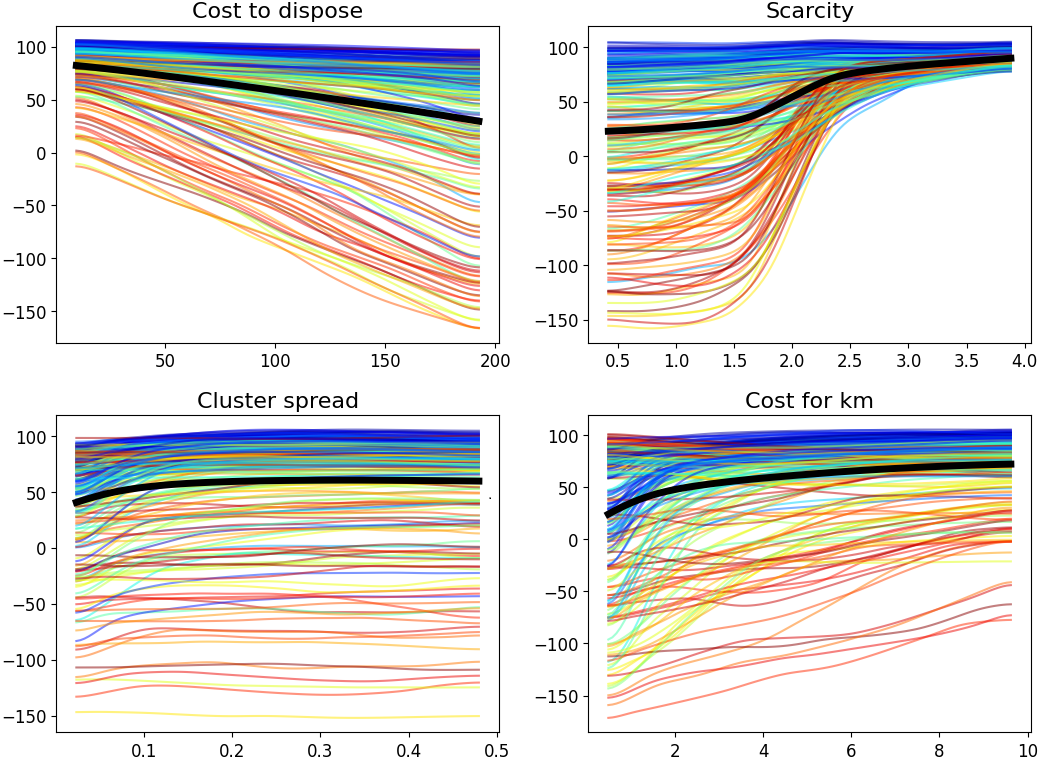
\includegraphics[width=0.9\textwidth, height=0.5\textheight, keepaspectratio]{Images/cireco_pdp_ice_density_price.png}
      \begin{itemize}
          \item Macroscopic rupture: Prediction collapses/diverges at specific parameter thresholds (e.g., density).
      \end{itemize}
    \end{column}
    \begin{column}{0.5\textwidth}
      \centering
      \textbf{Explanatory Space (Schelling SHAP)} \\
      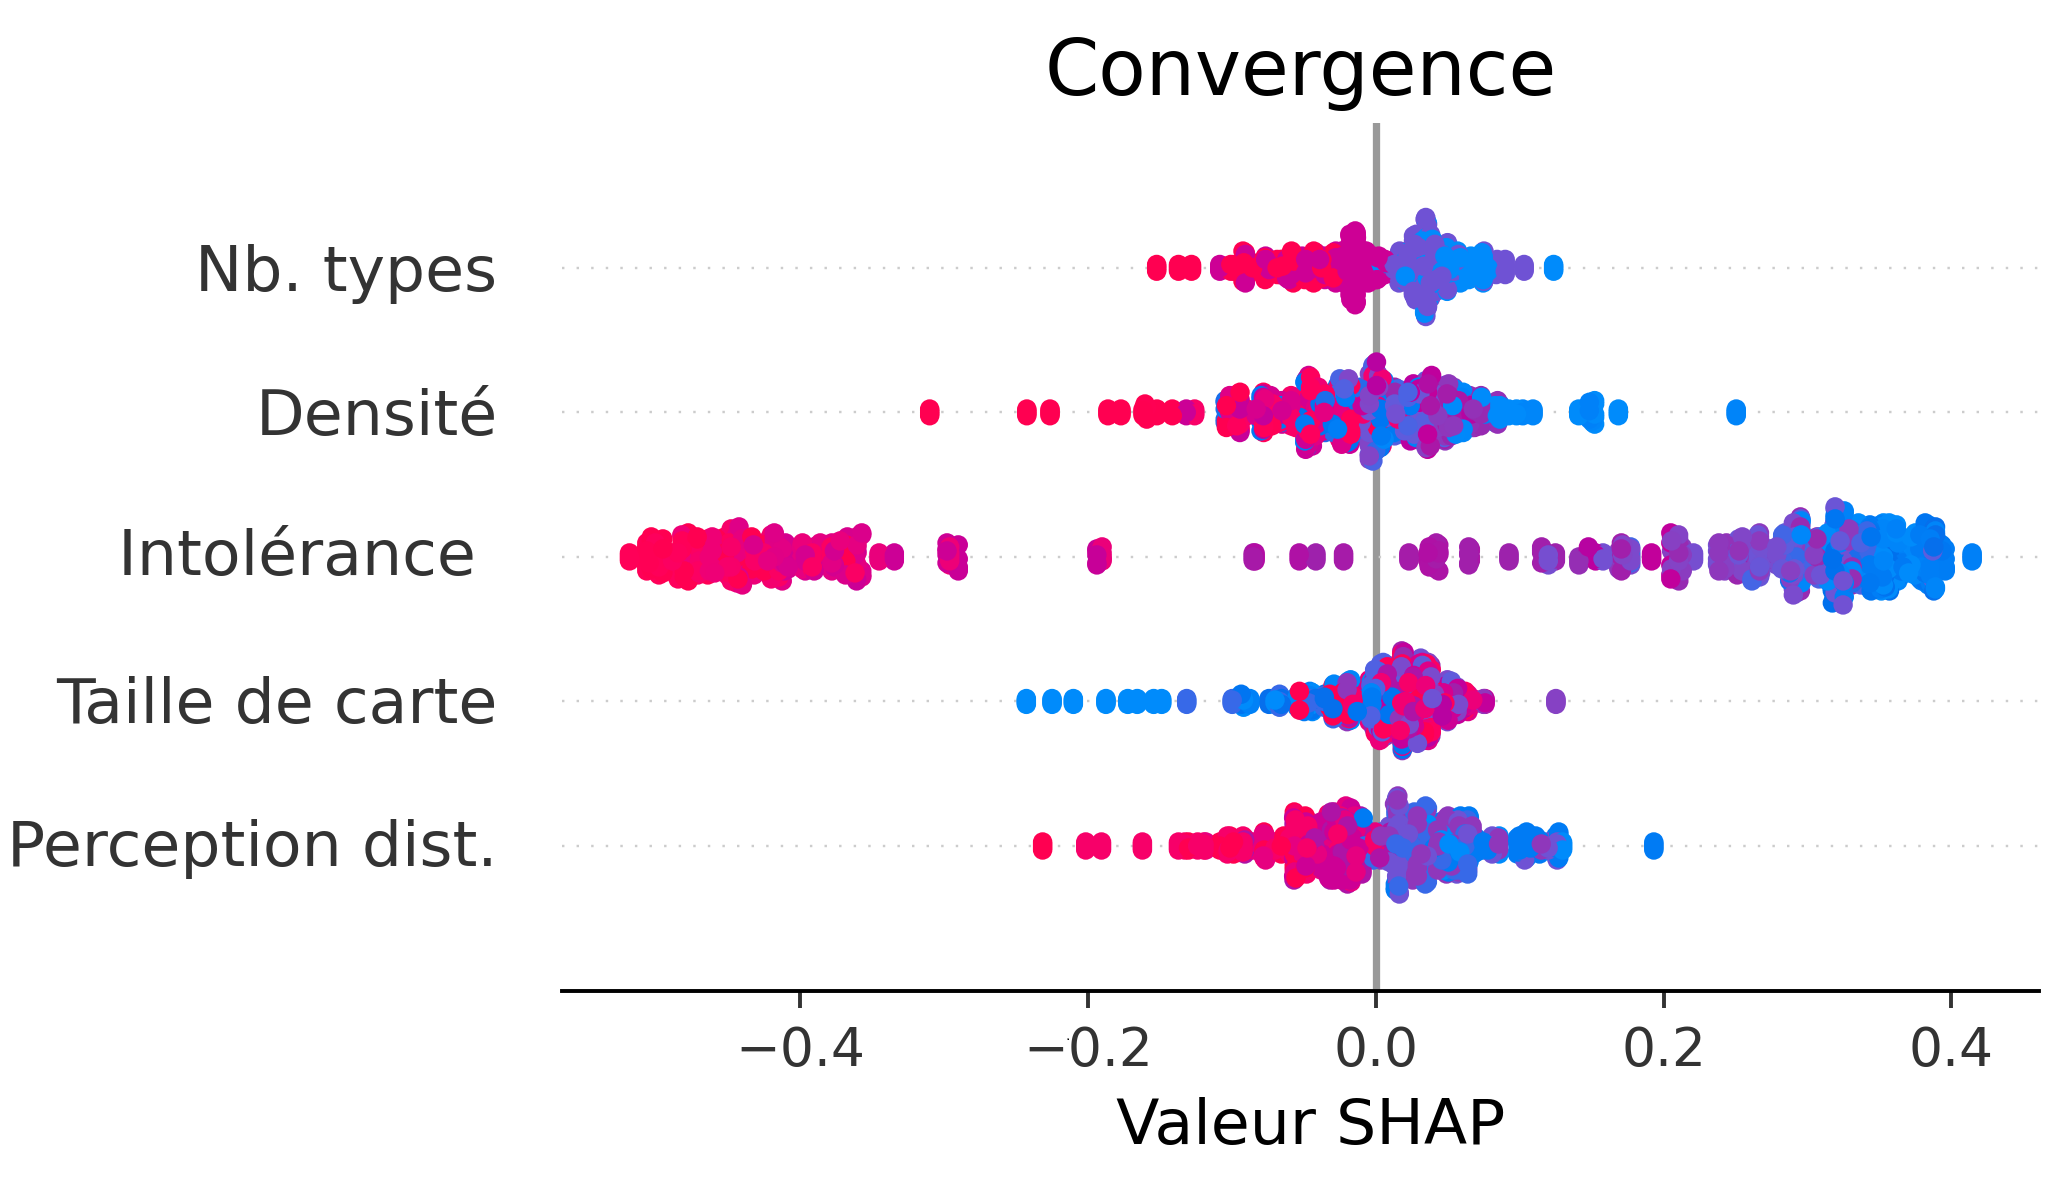
\includegraphics[width=0.9\textwidth, height=0.5\textheight, keepaspectratio]{Images/shap_RF_conv(1).png}
      \begin{itemize}
          \item Internal logic shift: Appearance of isolated "islands" where features suddenly dominate convergence.
      \end{itemize}
    \end{column}
  \end{columns}
  
  \vspace{0.3cm}
  \textit{Conclusion: Hunting for explanatory novelty guarantees finding physical tipping points.}
\end{frame}

\begin{frame}[fragile]{The Core Concept: Explanatory Diversity}
  \textbf{The Shift:} Stop hunting for \textit{prediction uncertainty}; start hunting for \textit{explanatory novelty}.
  
  \vspace{0.5cm}
  Instead of looking only at the prediction $y$, we extract feature contribution profiles using Explainable AI (SHAP):
  $$S(x) = \text{SHAP}(f, x)$$
  
  \textbf{The Goal:} Explicitly sample regions where the internal logic (the explanation) of the model fundamentally changes.
\end{frame}

\section{Pipeline \& Innovations}

\begin{frame}[fragile]{The Active Learning Pipeline Architecture}
  \begin{figure}
      \centering
      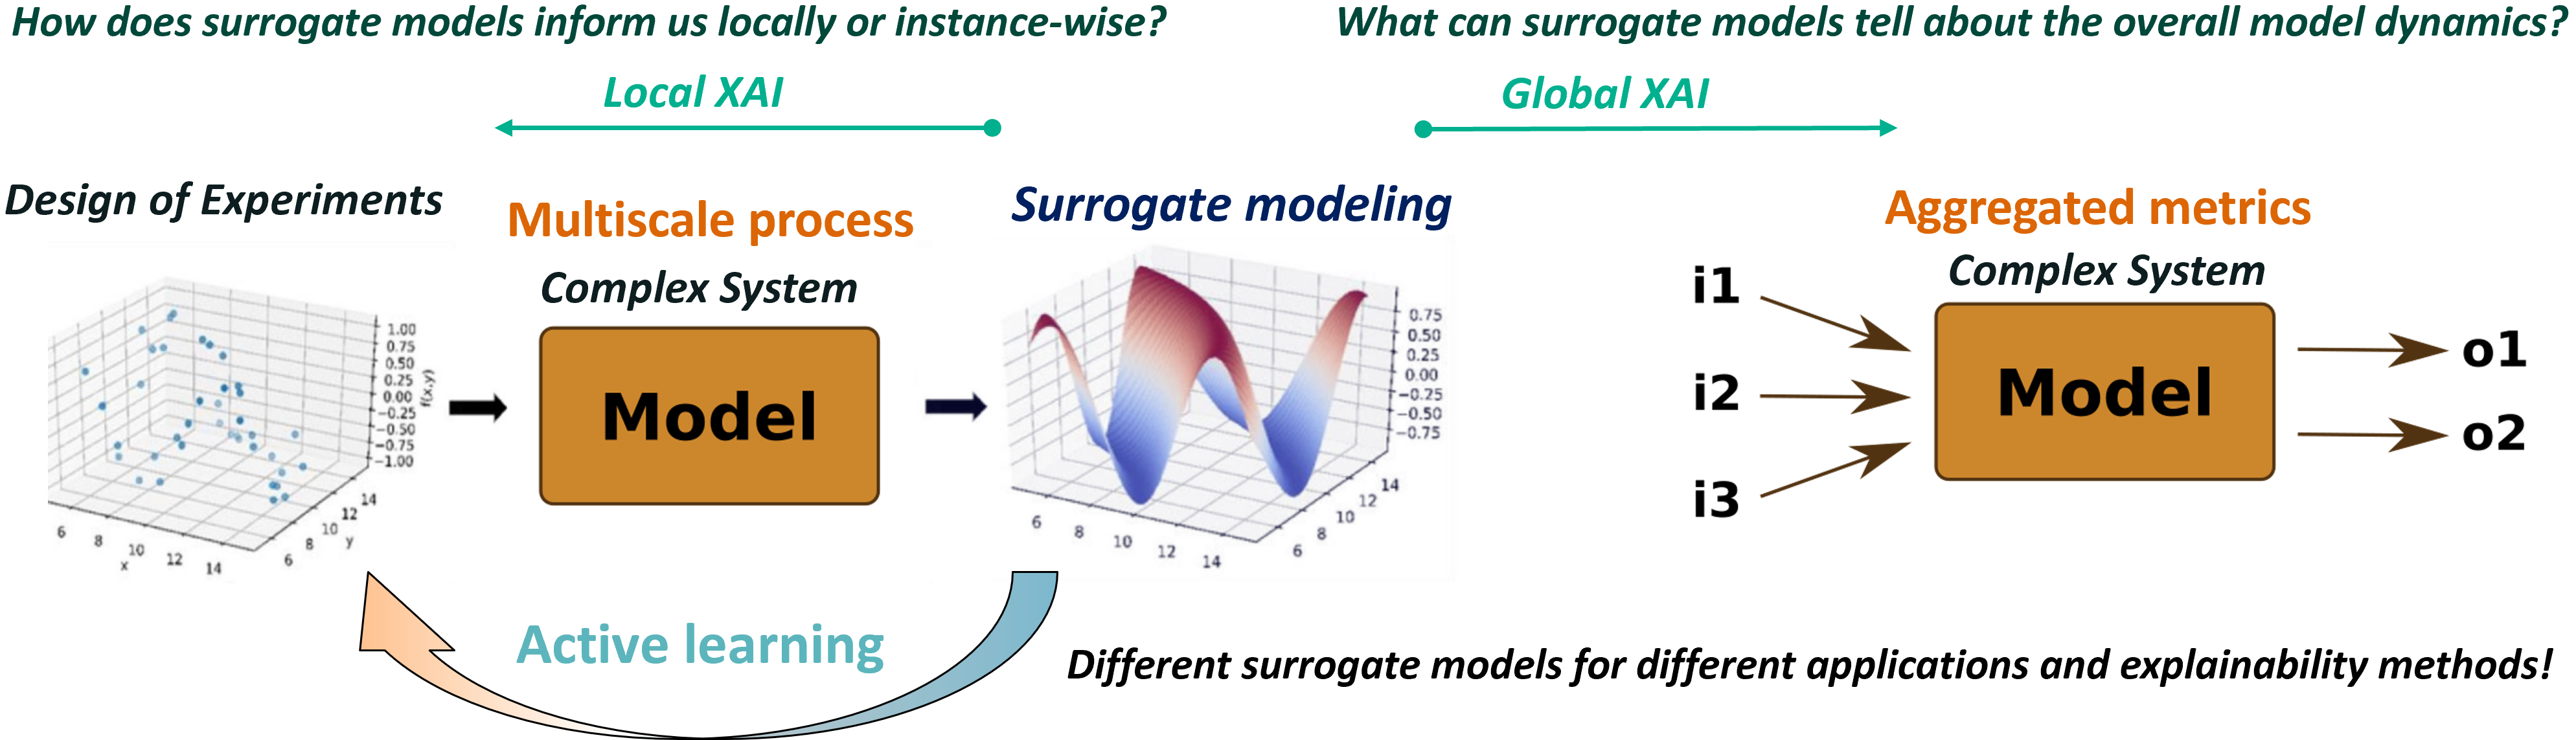
\includegraphics[width=0.9\textwidth, height=0.75\textheight, keepaspectratio]{Images/pipeline.png}
      \caption{Flowchart of the Proposed Active Learning Framework}
  \end{figure}
\end{frame}

\begin{frame}[fragile]{Algorithmic Innovations (I): Fast Cosine Proxy}
  \textbf{From Slow KDE to Fast Cosine Proxy:}
  \begin{itemize}
      \item The initial theory relied on high-dimensional Kernel Density Estimation (KDE) on SHAP values:
      $$p_{SHAP}(S(x)) = \frac{1}{N} \sum_{i=1}^N K_h(S(x) - S(x_i))$$
      \item \textbf{The Upgrade:} KDE suffers from the curse of dimensionality and is computationally prohibitive.
      \item \textbf{The Solution:} We implemented a \textbf{Fast Density Proxy via Cosine Distance} (Nearest Neighbors) in SHAP space. High cosine distance translates directly to high explanatory novelty.
  \end{itemize}
\end{frame}

\begin{frame}[fragile]{Algorithmic Innovations (II): Bi-Objective Optimization}
  \textbf{Framing Dynamic-US as a Bi-Objective Problem:}
  
  Rather than a static heuristic, the acquisition strategy sweeps a Pareto front to simultaneously:
  \begin{enumerate}
      \item \textbf{Maximize Physical Exploration:} Predictive variance in input space ($\sigma^2_{GP}$).
      \item \textbf{Maximize Explanatory Exploitation:} Novelty via Cosine distance in SHAP space ($\text{EI}_{MFK}$).
  \end{enumerate}
  
  $$a_{Dynamic}(x) = (1 - \alpha^{(t)}) \cdot \widetilde{\sigma}^2_{GP}(x) + \alpha^{(t)} \cdot \widetilde{\text{EI}}_{MFK}(S(x))$$
  
  \begin{itemize}
      \item Over iterations, $\alpha^{(t)}$ shifts dynamically from $0.0 \to 1.0$.
      \item \textbf{Result:} It maps the macroscopic behavior first, then pivots to isolate the complex \textbf{tipping points}.
  \end{itemize}
\end{frame}

\section{Results \& Analysis}

\begin{frame}[fragile]{Hunting Tipping Points in PCA Space}
  \begin{columns}
    \begin{column}{0.4\textwidth}
      \begin{itemize}
        \item Traditional methods (LHS, Space-US) sample densely in the homogeneous bulk.
        \item Our method (\textbf{SHAP-US} and \textbf{Dynamic-US}) efficiently populates the boundaries and critical tipping points.
      \end{itemize}
    \end{column}
    \begin{column}{0.6\textwidth}
      \begin{figure}
        \centering
        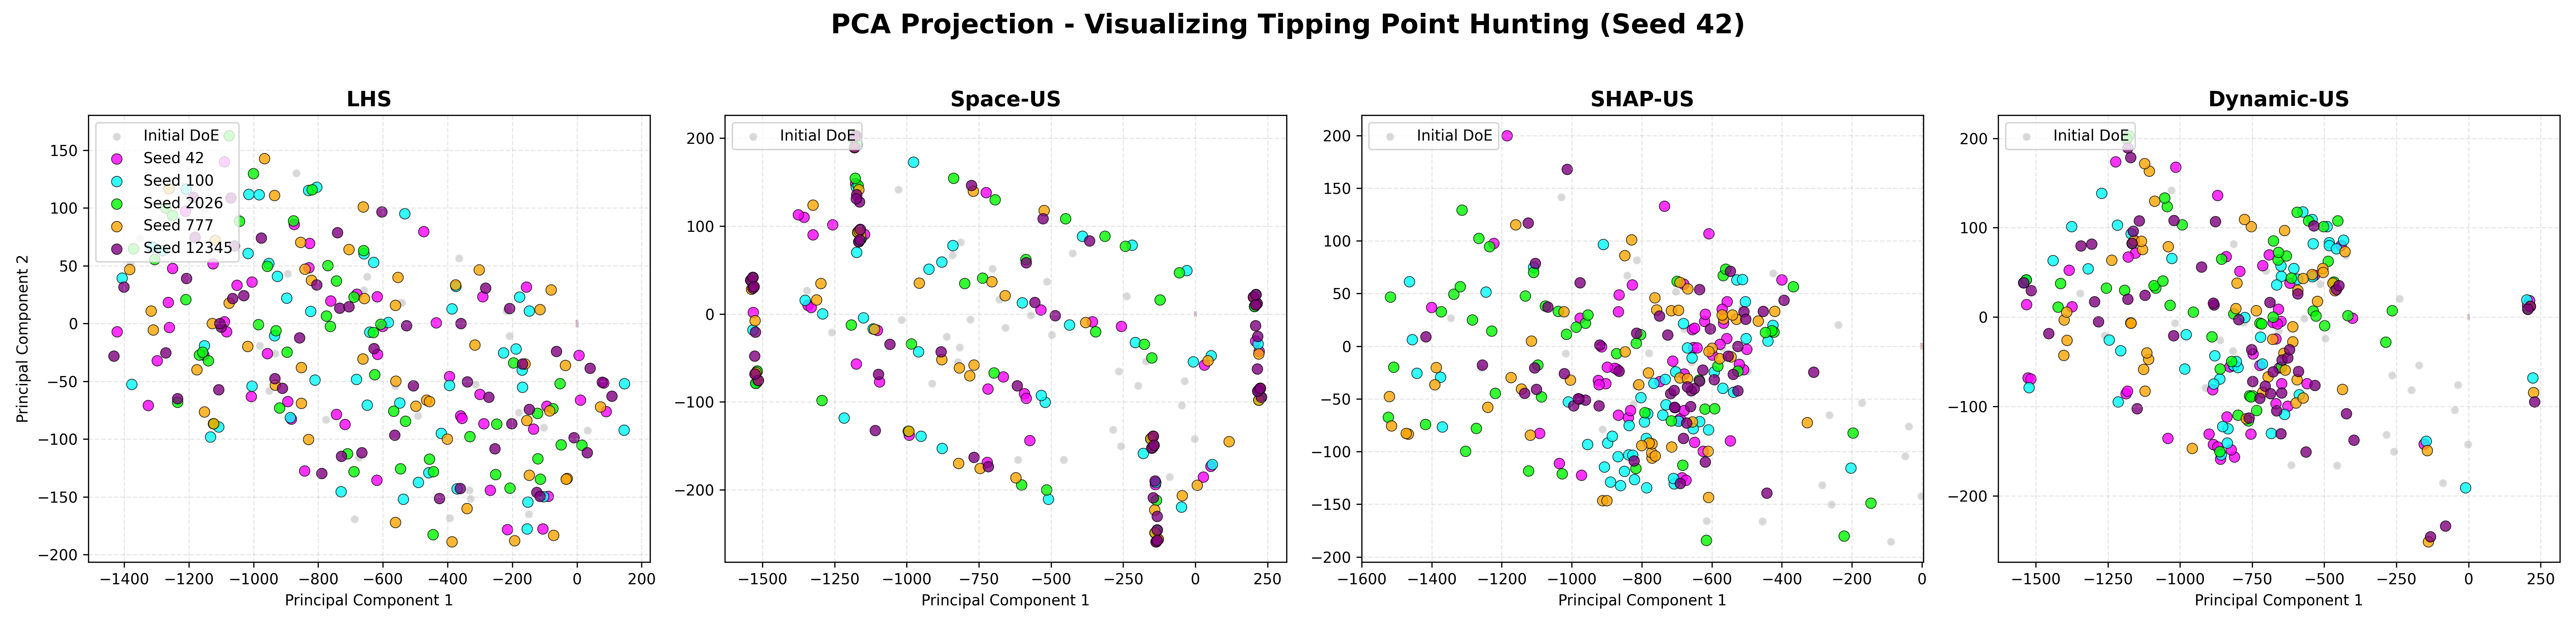
\includegraphics[width=\textwidth]{Images/cireco_final_tipping_points_pca.png}
        \caption{Exploration of the Cireco Model (PCA space)}
      \end{figure}
    \end{column}
  \end{columns}
\end{frame}

\begin{frame}[fragile]{Convergence and Stability over Time}
  \begin{columns}
    \begin{column}{0.5\textwidth}
      \begin{figure}
        \centering
        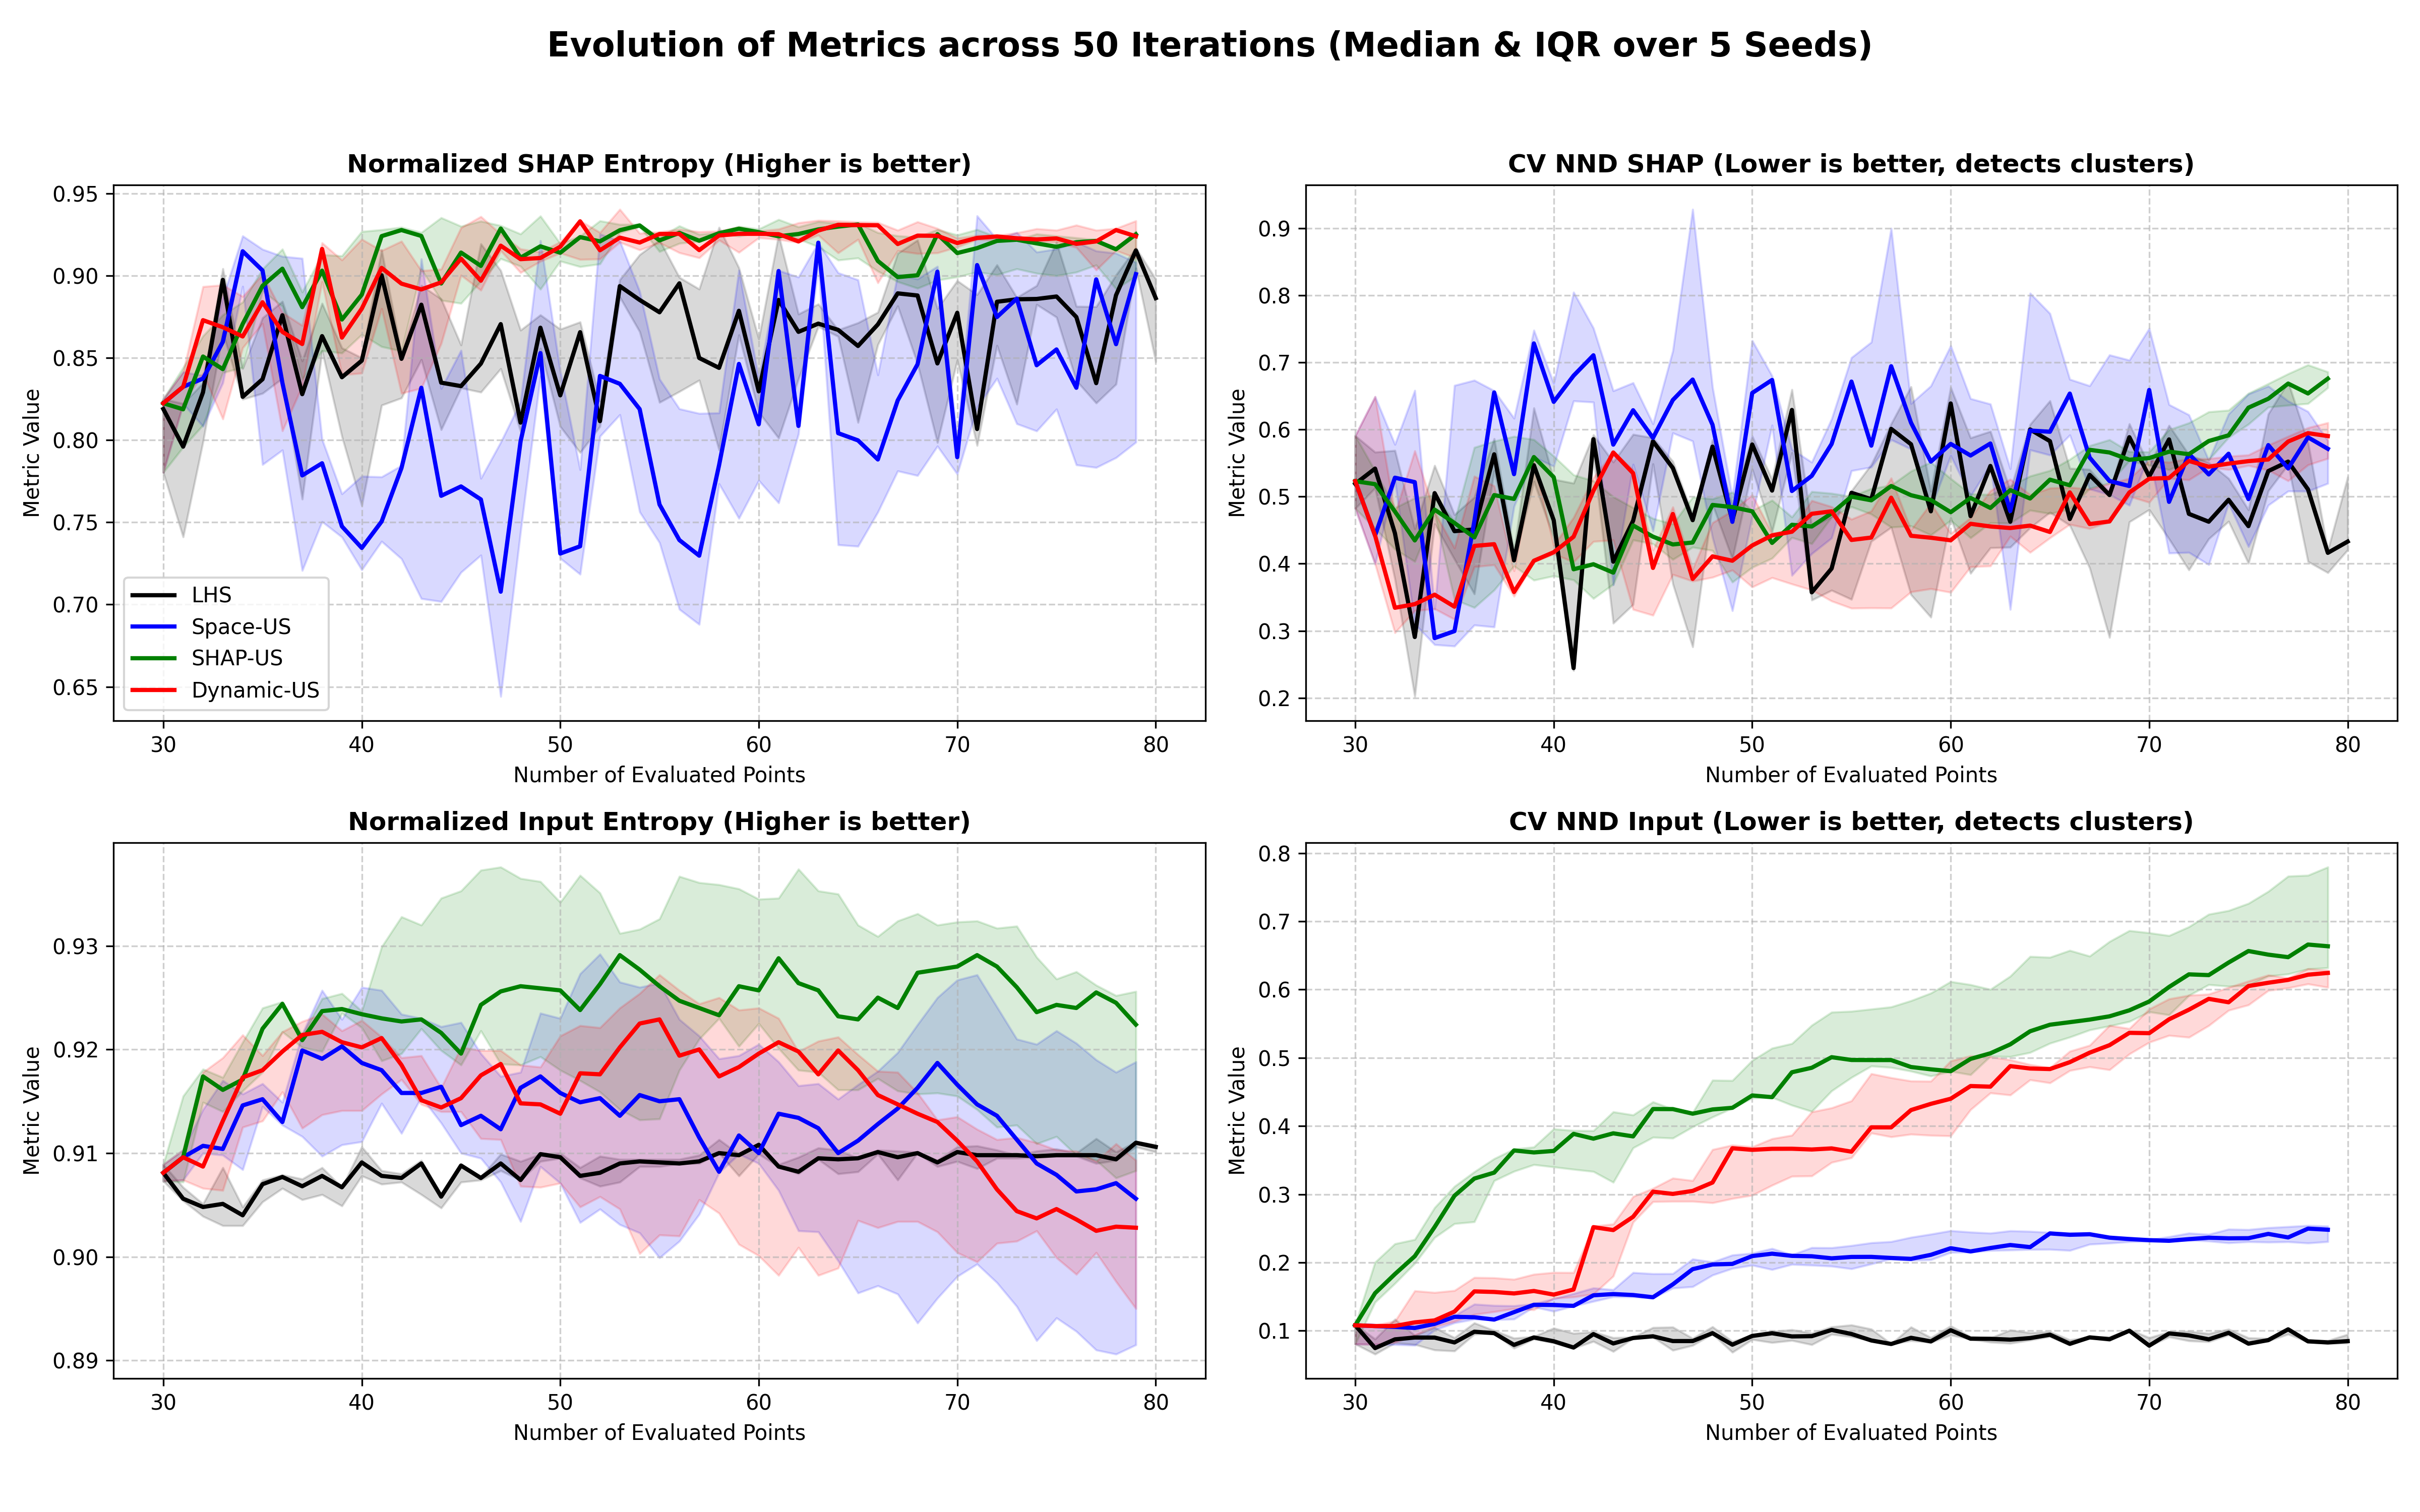
\includegraphics[width=0.9\textwidth, height=0.7\textheight, keepaspectratio]{Images/schelling_final_all_metrics_evolution.png}
      \end{figure}
    \end{column}
    \begin{column}{0.5\textwidth}
      \begin{itemize}
        \item \textbf{Dynamic-US (Red)} matches the high explanatory diversity (SHAP entropy) of SHAP-US.
        \item Crucially, it avoids the catastrophic crash in physical input entropy seen in pure SHAP-US.
        \item It converges reliably without pathological spatial clustering.
      \end{itemize}
    \end{column}
  \end{columns}
\end{frame}

\begin{frame}[fragile]{Under the Hood: How Dynamic-US Samples Differently}
  \begin{columns}
    \begin{column}{0.5\textwidth}
      \begin{figure}
        \centering
        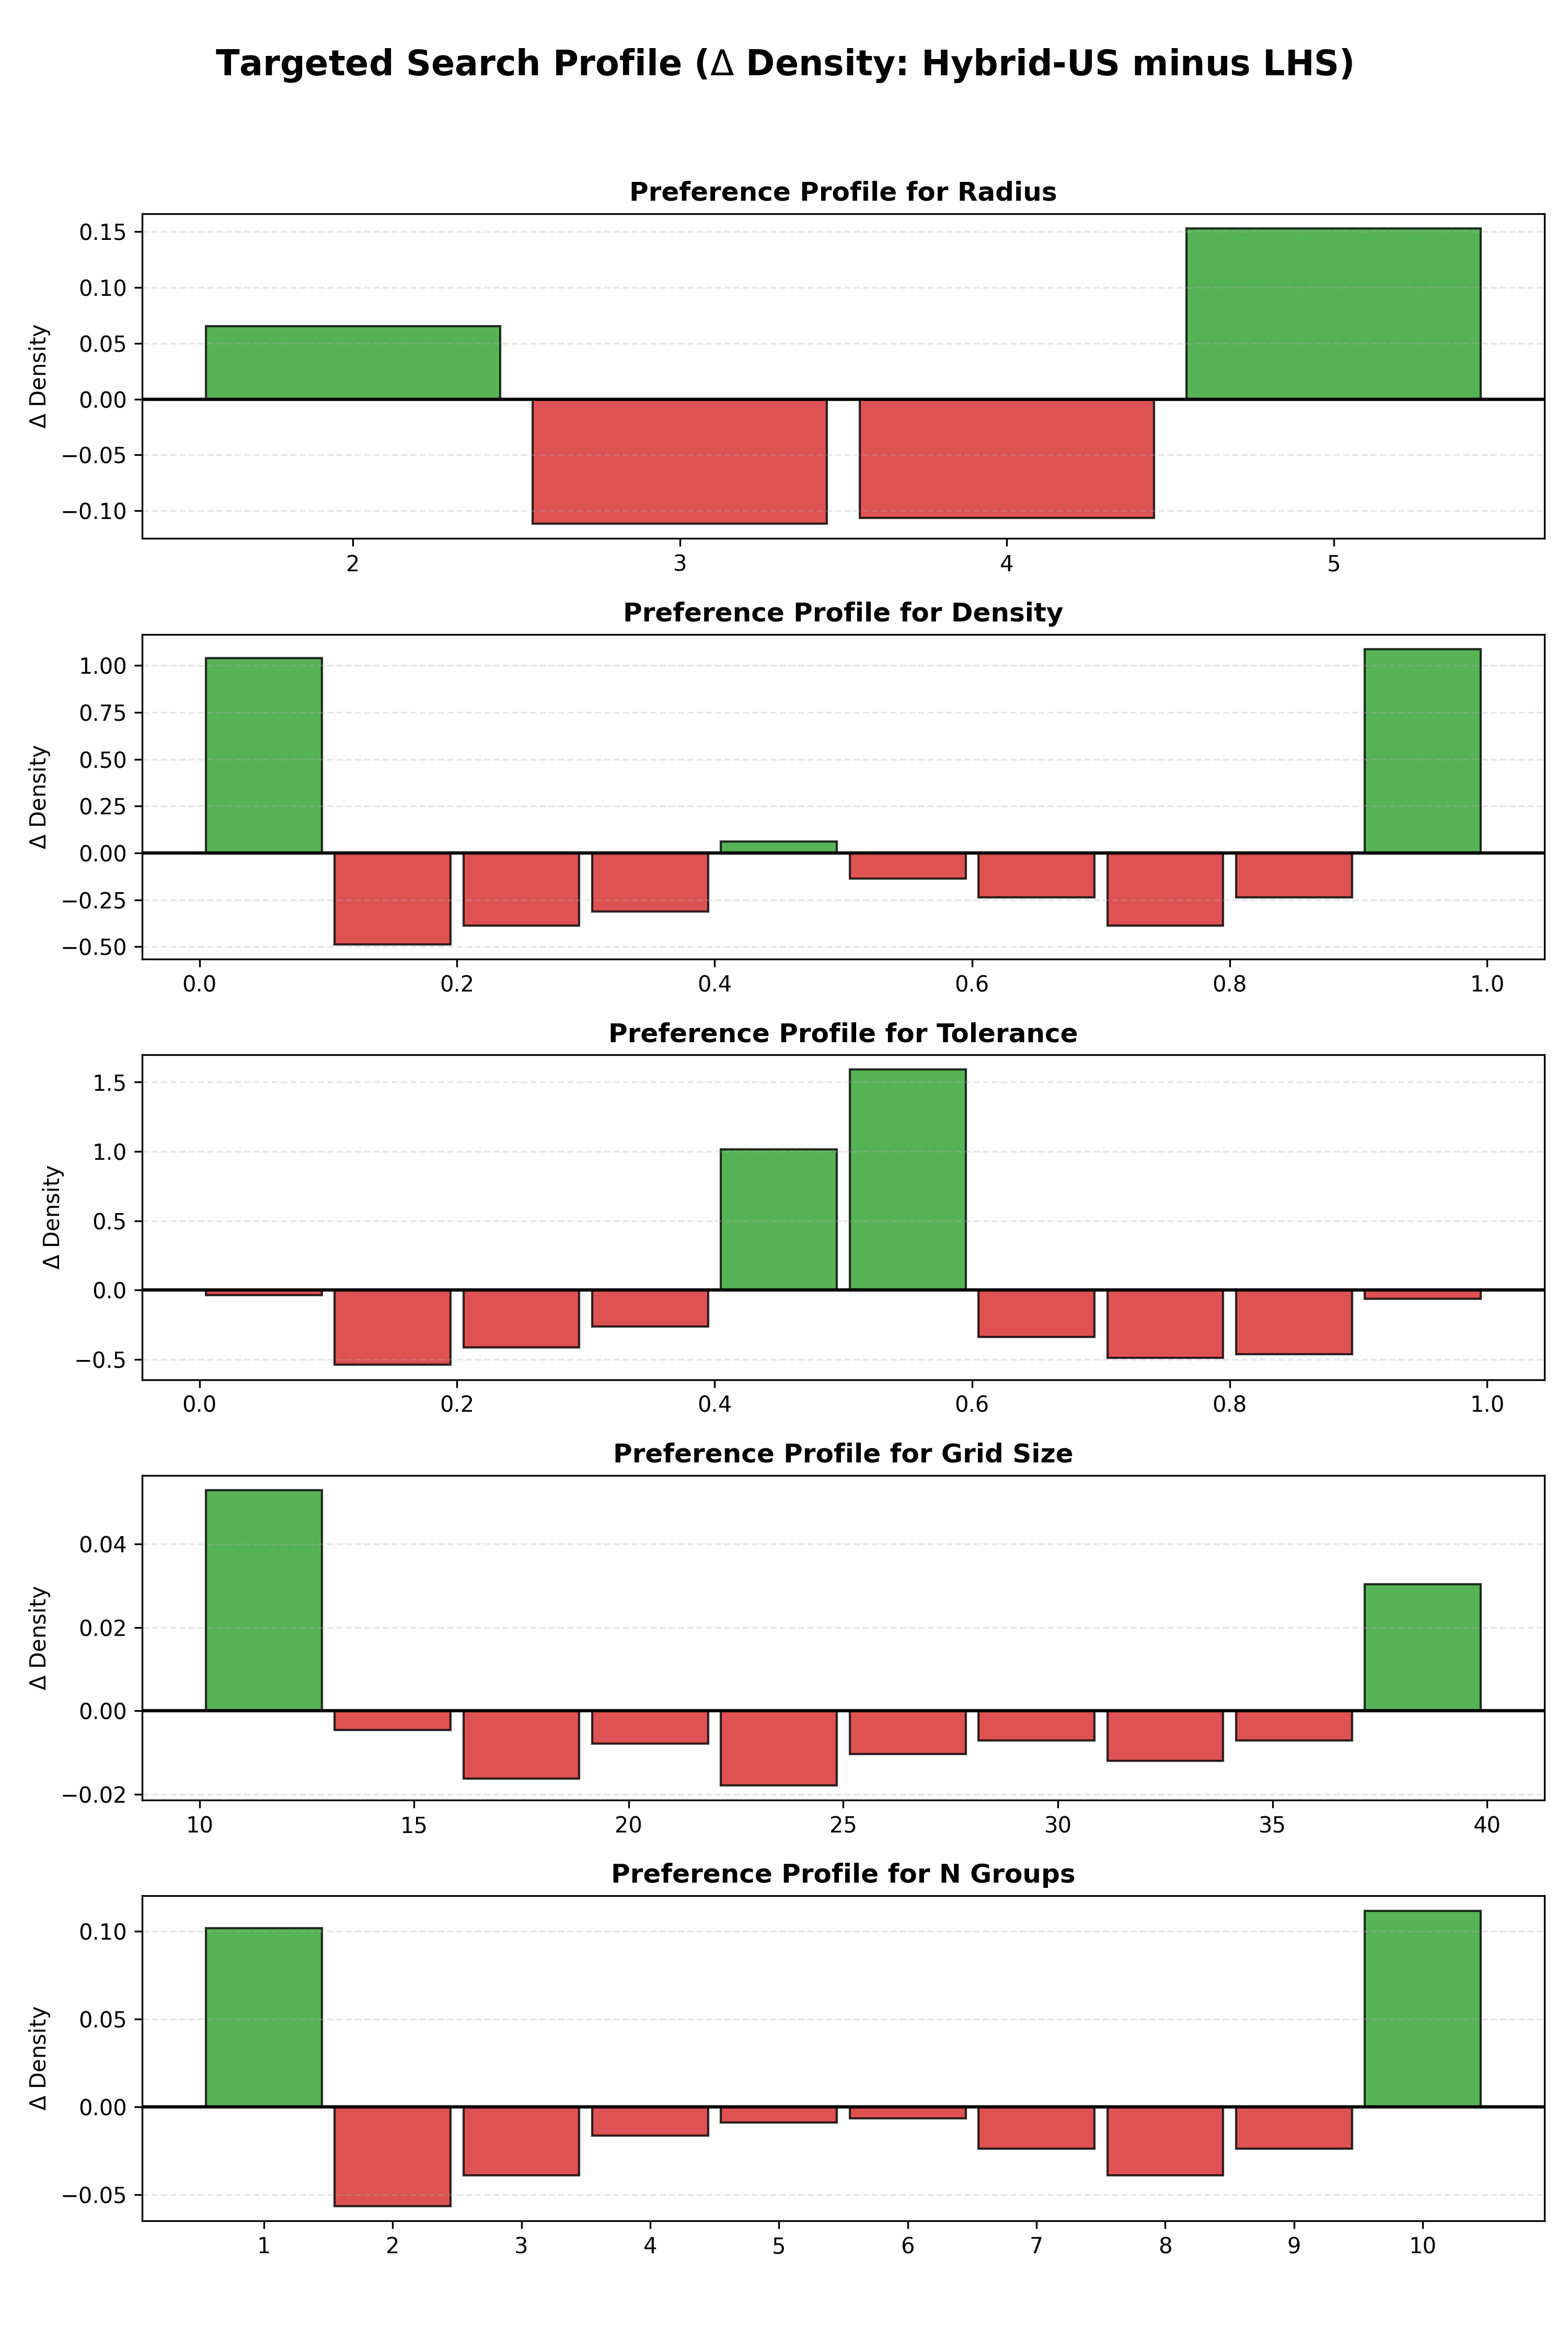
\includegraphics[width=0.9\textwidth, height=0.7\textheight, keepaspectratio]{Images/schelling_final_hybrid_diff_profile.png}
      \end{figure}
    \end{column}
    \begin{column}{0.5\textwidth}
      \begin{itemize}
        \item Shows the Delta Density (\textbf{Dynamic-US minus LHS}).
        \item \textbf{Green:} Active learner intentionally over-sampled this region.
        \item \textbf{Red:} Actively ignored.
        \item Validates that Dynamic-US aggressively targets specific narrow bands (e.g., Tolerance around 0.5) where the tipping points live.
      \end{itemize}
    \end{column}
  \end{columns}
\end{frame}

\begin{frame}[fragile]{Dual Space Efficiency}
  \begin{columns}
    \begin{column}{0.4\textwidth}
      \begin{itemize}
        \item \textbf{Physical Diversity} vs \textbf{Explanatory Diversity}.
        \item Dynamic-US achieves a rapid gain in explanatory entropy, proving it discovers diverse causal mechanisms faster.
        \item Background dots represent 250 iterations across 5 seeds.
      \end{itemize}
    \end{column}
    \begin{column}{0.6\textwidth}
      \begin{figure}
        \centering
        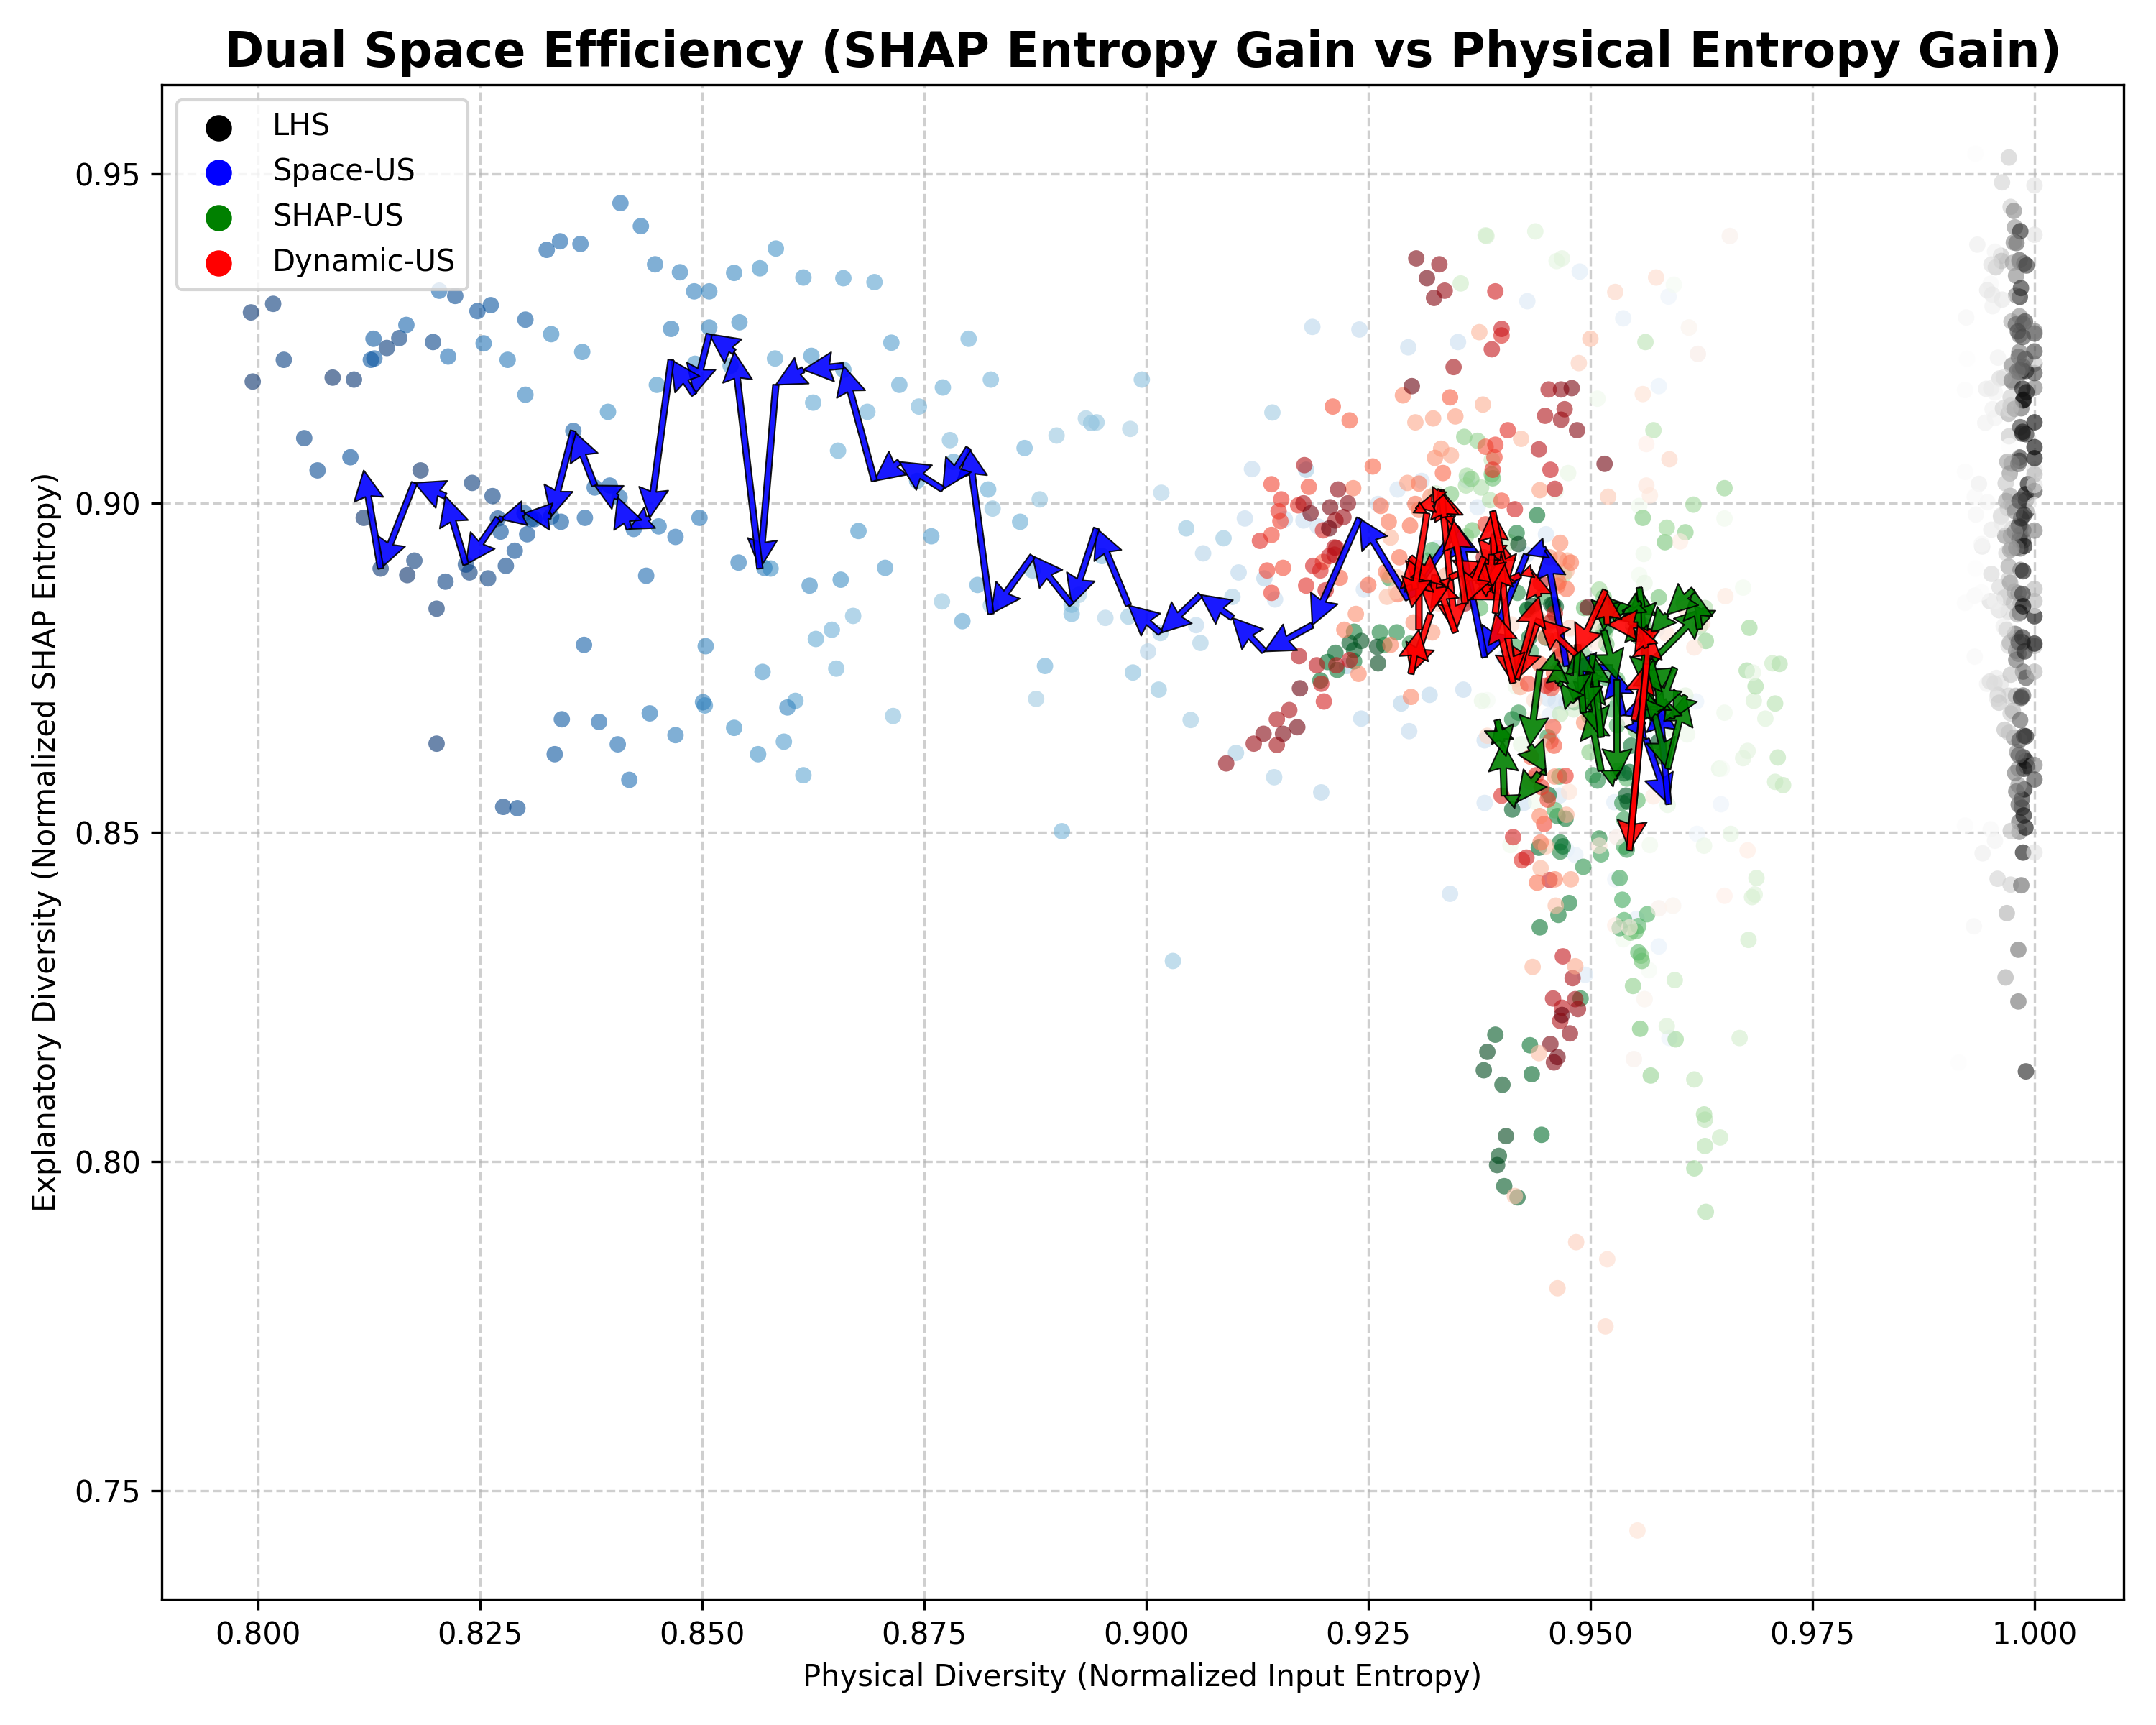
\includegraphics[width=\textwidth]{Images/cireco_final_dual_space_efficiency.png}
      \end{figure}
    \end{column}
  \end{columns}
\end{frame}

\section{Conclusion}

\begin{frame}{Conclusion \& Perspectives}
  \textbf{Contributions:}
  \begin{itemize}
      \item A model-agnostic, multi-fidelity XAI loop that achieves deep structural understanding rather than just raw predictive accuracy.
      \item Demonstrates that optimizing for explanatory diversity uncovers tipping points exponentially faster than classic DoE or SUR.
      \item Validated on robust Agent-Based Models (Cireco, Schelling).
  \end{itemize}
\end{frame}
  
\begin{frame}{Perspectives \& Future Work (I)}
  \textbf{Scaling the Optimization and Dimensionality:}
  \begin{itemize}
      \item \textbf{Integrated Variance Reduction (IMSE):} Replacing pointwise GP variance ($\sigma^2_{GP}$) with Integrated Mean Squared Error to solve the extrapolation artifacts at the boundaries of the hypercube.
      \item \textbf{Active Subspace Projection:} Mathematically linking SHAP tracking to the dynamic rotation of the Active Subspace. This provides a theoretical pathway to scale to $M > 15$ dimensions by reducing ExactSHAP overhead.
      \item \textbf{Native Simulator Integration:} Transitioning the surrogate methodology from the MLP proxy directly to the computationally intensive ABM cores.
  \end{itemize}
\end{frame}

\begin{frame}{Perspectives \& Future Work (II)}
  \textbf{Advanced Surrogate \& Acquisition Optimization:}
  \begin{itemize}
      \item \textbf{Multi-Objective DFO (EHVI):} Replacing linear scalarization with Expected Hypervolume Improvement to capture non-convex regions of the Pareto front.
      \item \textbf{Trust-Region Bayesian Optimization (TuRBO):} Using dynamically sized local trust regions to handle the inherently non-stationary landscapes of SHAP novelty.
      \item \textbf{Global Solvers (CMA-ES):} Upgrading the acquisition optimizer from L-BFGS-B to Covariance Matrix Adaptation Evolution Strategy to avoid local minima traps in the multimodal novelty surface.
  \end{itemize}
\end{frame}

\begin{frame}[standout]
  Questions?
\end{frame}

\end{document}
